\chapter{Implementation Details}
\label{ch:implementation}

This chapter documents the concrete software engineering implementation of CodeQuest AI across the Unity~6 client, the FastAPI backend services, the Docker evaluation sandbox, the PostgreSQL database, and Keycloak authentication.

\section{Software Technology Stack}
Table~\ref{tab:tech_stack} details the comprehensive technology stack employed across the subsystems:

\begin{table}[htbp]
\centering
\small
\renewcommand{\arraystretch}{1.25}
\caption{CodeQuest AI Software Technology Stack}
\label{tab:tech_stack}
\begin{tabularx}{\textwidth}{|p{0.26\textwidth}|p{0.38\textwidth}|X|}
\hline
\rowcolor{gray!25}\textbf{Component} & \textbf{Technology / Library} & \textbf{Version / Environment} \\ \hline
\textbf{Game Client} & Unity Engine (C\#, .NET Standard 2.1) & 6000.3.19f1 (Unity 6 URP) \\ \hline
\textbf{Render Pipeline} & Universal Render Pipeline (URP) & Forward+ Path, D3D12 \\ \hline
\textbf{Client UI Framework} & Unity uGUI + TrueType Font Loader & Arial / Consolas Assets \\ \hline
\textbf{Backend Gateway} & FastAPI (Python 3.11 async) & Uvicorn ASGI on port 8000 \\ \hline
\textbf{Relational Database} & PostgreSQL & 17.5-alpine container \\ \hline
\textbf{ORM \& Migrations} & SQLAlchemy 2.0 + Alembic & Async engine (asyncpg) \\ \hline
\textbf{Execution Worker} & Docker + Python Execution Engine & Port 8100 (Evaluator) \\ \hline
\textbf{Identity Provider} & Keycloak (OIDC / OAuth 2.0 PKCE) & \texttt{codequest-dev} on 8080 \\ \hline
\textbf{Character Assets} & Kenney Stylized 3D Modular Character & Humanoid Avatar \& Controller \\ \hline
\end{tabularx}
\end{table}

\section{Unity 3D Game Client Implementation}

\subsection{Third-Person Character Controller and Motor}
Player traversal is managed by \texttt{ThirdPersonMotor.cs}, which utilizes a Unity \texttt{CharacterController} component. The motor processes input vectors in camera-relative space, computes smooth yaw rotations via spherical linear interpolation (\texttt{Quaternion.Slerp}), and simulates gravity, sprint acceleration, and vertical jumping. The character visual is driven by an \texttt{Animator} component with an explicit Humanoid Avatar configuration mapping idle, running, and jumping states. Figure~\ref{fig:variable_valley_gameplay} displays the rendered 3D Variable Valley game world showing the player avatar, navigational beacons, and guide NPCs (Signal Keeper and Mira).

\begin{figure}[htbp]
    \centering
    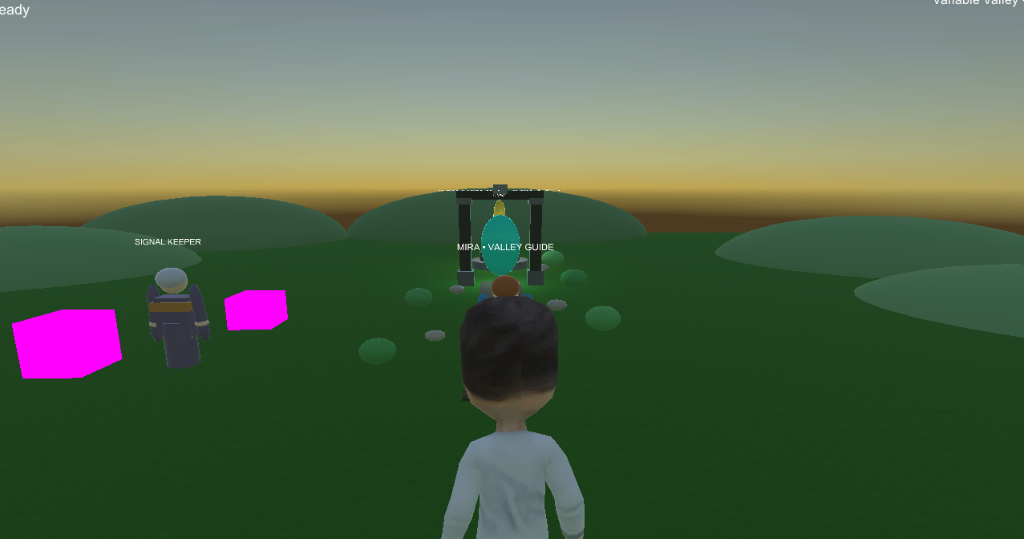
\includegraphics[width=0.88\textwidth]{figures/variable_valley_gameplay.png}
    \caption{Variable Valley 3D Game World with Player Avatar, Environmental Beacons, and NPCs}
    \label{fig:variable_valley_gameplay}
\end{figure}

\subsection{Typography and the Unity 6 Standalone Font Fix}
During standalone deployment on Unity~6, a critical runtime issue was diagnosed where standard UI buttons rendered as solid blank blue rectangles. Investigation revealed that Unity~6 no longer bundles the legacy \texttt{LegacyRuntime.ttf} resource in standalone Windows builds; calls to \texttt{Resources.GetBuiltinResource<Font>("LegacyRuntime.ttf")} returned \texttt{null}, causing the UI text renderer to generate zero mesh vertices.

To resolve this defect, dedicated TrueType font assets were imported into \texttt{Assets/Resources/}:
\begin{itemize}
    \item \textbf{UI Font (\texttt{CodeQuestFont.ttf}):} Arial TrueType font for HUD titles, buttons, instructions, and dialogue labels.
    \item \textbf{Monospace Font (\texttt{CodeQuestMono.ttf}):} Consolas TrueType font for multiline code input, indentation formatting, and evaluation terminal output.
\end{itemize}
Static cached loaders (\texttt{GetUiFont()} and \texttt{GetMonoFont()}) were implemented in \texttt{RuntimeHud.cs} with dynamic fallback resolution chains to operating system fonts (\texttt{Segoe UI}, \texttt{Arial}, \texttt{Cascadia Code}), guaranteeing robust font instantiation across all execution environments.

\subsection{Heads-Up Display and Coding Modal Interface}
The UI is constructed programmatically in \texttt{RuntimeHud.cs} via a screen-space overlay canvas. As shown in Figure~\ref{fig:ui_editor_annotated}, the coding modal is organized into three distinct visual regions:
\begin{enumerate}
    \item \textbf{Header \& Instruction Bar:} Displays the active challenge banner (\texttt{"Variable Valley --- Challenge 1"}) and clear problem descriptions.
    \item \textbf{Python Editor Card:} An interactive \texttt{InputField} with \texttt{LineType.MultiLineNewline}, dark navy background (\texttt{\#0a0f18}), and Consolas typography.
    \item \textbf{Control Actions \& Output Card:} Features a prominent green \texttt{"$\blacktriangleright$ Run / Submit"} button, a dark \texttt{"Close"} button, and an emerald-accented \texttt{"Output / Test Results"} card displaying real-time test execution results.
\end{enumerate}

\begin{figure}[htbp]
    \centering
    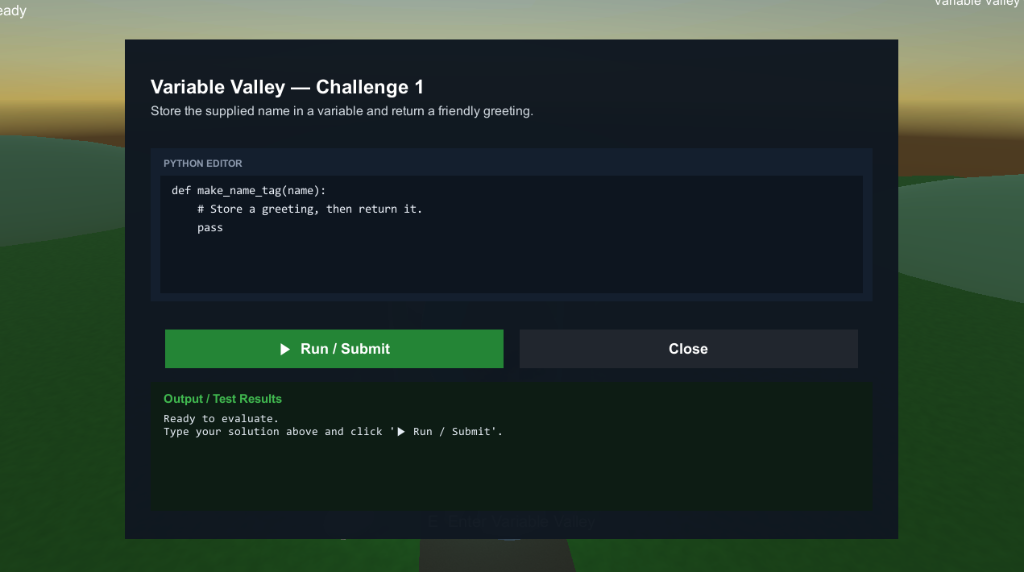
\includegraphics[width=0.88\textwidth]{figures/python_challenge_editor.png}
    \caption{Annotated In-Game Python Challenge Interface in Variable Valley}
    \label{fig:ui_editor_annotated}
\end{figure}

\section{Backend Gateway and Service Architecture}
The backend service (\texttt{BackendAPI}) is organized following clean architectural principles:
\begin{itemize}
    \item \texttt{routers/}: Modular FastAPI endpoint controllers for health checks, curriculum catalogs, quest updates, and challenge submissions.
    \item \texttt{services/}: Business logic services orchestrating quest prerequisites, progress calculation, and evaluator job dispatching.
    \item \texttt{models/}: Declarative SQLAlchemy models defining relational tables and relationships.
    \item \texttt{schemas/}: Pydantic validation models enforcing strict JSON schemas for incoming and outgoing HTTP payloads.
\end{itemize}

Listing~\ref{lst:submission_job} illustrates the structured evaluation job schema dispatched between the FastAPI gateway and the Docker execution worker:

\begin{lstlisting}[language=Python, caption={Structured Evaluation Job Schema Dispatched to Worker}, label={lst:submission_job}, basicstyle=\ttfamily\footnotesize, frame=single]
job = {
    "submissionId": str(uuid.uuid4()),
    "challengeSlug": "valley-name-tag",
    "challengeVersion": 1,
    "evaluatorVersion": "sha256:09509b92db75...",
    "source": source_code_text,
    "sourceDigest": hashlib.sha256(source_code_text.encode()).hexdigest(),
    "definition": {
        "mode": "function",
        "functionName": "make_name_tag",
        "visibleTests": [
            {"input": ["Ada"], "expected": "Hello, Ada!"},
            {"input": ["Kai"], "expected": "Hello, Kai!"}
        ],
        "hiddenTests": [
            {"input": ["Grace"], "expected": "Hello, Grace!"}
        ],
        "timeLimitMs": 5000,
        "outputLimitBytes": 65536
    }
}
\end{lstlisting}

\section{Sandboxed Execution Worker Implementation}
The Python Execution Service (\texttt{PythonExecutionService}) provides a hardened microservice on port 8100. When receiving a submission, the worker:
\begin{enumerate}
    \item Authenticates the gateway request using a pre-shared bearer token.
    \item Spawns an ephemeral container or isolated subprocess utilizing \texttt{codequest-evaluator:local}.
    \item Executes the target script against both visible and hidden test parameters using a custom test runner.
    \item Traps syntax errors, unhandled runtime exceptions, and assertion mismatches, packaging them into standardized diagnostic codes (\texttt{syntax\_error}, \texttt{runtime\_error}, \texttt{assertion\_failure}).
    \item Discards the execution container immediately upon completion to prevent state retention or cross-contamination.
\end{enumerate}

\section{Authentication and Security Architecture}
Identity management is anchored by Keycloak running on port 8080. The game client utilizes the OAuth~2.0 Authorization Code flow with Proof Key for Code Exchange (PKCE), opening an ephemeral local loopback HTTP server to receive the authorization code. Access tokens are transmitted via the standard \texttt{Authorization: Bearer <token>} header. All backend endpoints validate the cryptographic token signature against Keycloak's public JSON Web Key Set (JWKS).
